\documentclass[14pt,a4paper]{extarticle}
\usepackage[utf8]{inputenc}
\usepackage{amsmath, amssymb}
\usepackage{listings}
\usepackage{xcolor}
\usepackage{tcolorbox}
\usepackage{geometry}
\usepackage{titlesec}
\usepackage{enumitem}

% ---------- Graphics and TikZ ----------
\usepackage{tikz}
\usetikzlibrary{arrows.meta, positioning} % for nice arrowheads and node placement

%%%%%%%%%%% Prevent line breaking in pseudocode like %%%%%%%%%%
\lstset{keepspaces=true}

%%%%%%%%%%%% Correctiong Tables %%%%%%%%%%%%%%5
\usepackage{array}         % for custom column types
\usepackage{ragged2e}      % optional for better alignment
\usepackage{tabularx}      % Add this in your preamble

\geometry{margin=1in}

%%%%%%%%%%%%%%%%%%%%%%%%%%%% Title %%%%%%%%%%%%%%%%%%%%%%%%%%%%5
\titleformat{\section}{\normalfont\Large\bfseries}{\thesection.}{0.5em}{}
\titleformat{\subsection}{\normalfont\large\bfseries}{\thesubsection}{0.5em}{}

%%%%%%%%%%%%%%%%%%%%%%%% Pseudocode %%%%%%%%%%%%%%%%%%%%%%%%%%%%55
\usepackage{algorithm}
\usepackage{algpseudocode}
\usepackage{float}       % For [H] option to fix algorithm position
\algrenewcommand\algorithmicend{\textbf{end}}


\definecolor{codegray}{gray}{0.95}
\lstdefinestyle{pseudocode}{
  backgroundcolor=\color{codegray},
  basicstyle=\ttfamily\small,
  frame=single,
  showstringspaces=false,
  keywordstyle=\color{blue}\bfseries,
  commentstyle=\color{gray},
  morekeywords={procedure, for, to, if, then, else, return, while}
}

%-------------------- Python 
% Code styling
\lstdefinestyle{python}{
  language=Python,
  basicstyle=\ttfamily\small,
  keywordstyle=\color{black},
  commentstyle=\color{black},
  stringstyle=\color{black},
  showstringspaces=false,
  numbers=left,
  numberstyle=\tiny\color{gray},
  breaklines=true,
  frame=single,
  tabsize=4,
  captionpos=b
}

%%%%%%%%%%%%%% Hyperlink in Table of Content %%%%%%%%%%%%%%%
\usepackage{hyperref}
% ---------- Hyperref Setup ----------
\hypersetup{
    colorlinks=true,
    linkcolor=black,
    urlcolor=cyan,
    citecolor=blue
}

%%%%%%%% Renaming Listing(after \listofalgorithms) to Python Programs %%%%%%%%%%%%%%
\renewcommand{\lstlistlistingname}{Python Programs}

\title{Shortest Path Algorithms: Bellman-Ford and Floyd-Warshall}
\author{Varun Kumar}
\date{\today}

\begin{document}
\maketitle
\tableofcontents
\listofalgorithms
\lstlistoflistings
\listoftables
\newpage

\section{Introduction: Shortest Path Problem}
The \textbf{Shortest Path Problem} involves finding the path between two nodes in a \textbf{weighted graph} such that the sum of the edge weights is minimized.

This problem has many real-world applications:
\begin{itemize}[leftmargin=1.5em]
  \item Network routing
  \item Road navigation
  \item Flight booking systems
  \item Dependency resolution
\end{itemize}

Depending on the type of graph and requirements, different algorithms are used:
\begin{itemize}[leftmargin=1.5em]
  \item \textbf{Single-source shortest path:} e.g., Dijkstra, Bellman-Ford
  \item \textbf{All-pairs shortest path:} e.g., Floyd-Warshall
  \item \textbf{Graphs with negative weights:} Bellman-Ford, Floyd-Warshall
\end{itemize}

%%%%%%%%%%%%%%%%%%%%%%%%%%%%%%%%%%%%%%%%%%%%%%%%%%%%%%%%%%%%%%%%%%%%%%%%%%%%%%%%%%%%%%%%%%%%%%%
%%%%%%%%%%%%%%%%%%%%%%%%%%%%%%% Bellman-Ford Algorithm% %%%%%%%%%%%%%%%%%%%%%%%%%%%%%%%%%%%%%%%
%%%%%%%%%%%%%%%%%%%%%%%%%%%%%%%%%%%%%%%%%%%%%%%%%%%%%%%%%%%%%%%%%%%%%%%%%%%%%%%%%%%%%%%%%%%%%%%
\newpage
\section{Bellman-Ford Algorithm}
\subsection{Purpose}
The Bellman-Ford algorithm finds the shortest path from a single source to all other vertices in a weighted graph. Unlike Dijkstra’s algorithm, Bellman-Ford works correctly even when the graph contains \textbf{negative edge weights}.

\subsection{Problem Context}
Given a directed graph $G = (V, E)$ with edge weights $w(u, v)$ (which may be negative), and a source vertex $s \in V$, compute the shortest path distance $d(s, v)$ for every $v \in V$. Also detect whether a \textbf{negative-weight cycle} is reachable from the source.

\subsection{Time Complexity}
\[
O(V \cdot E)
\]
where $V$ is the number of vertices and $E$ is the number of edges.

\subsection{Space Complexity}
\[
O(V)
\]
for storing the distance array.

\subsection{Key Features}
\begin{itemize}[leftmargin=1.5em]
  \item Works for directed and undirected graphs.
  \item Handles graphs with negative edge weights.
  \item Detects and reports negative weight cycles.
  \item Slower than Dijkstra’s algorithm, but more general.
\end{itemize}

\subsection{Step-by-Step Explanation}
\begin{enumerate}[leftmargin=1.5em]
  \item Initialize the distance to all vertices as $\infty$, except the source which is 0.
  \item Repeat $V - 1$ times:
  \begin{itemize}
    \item For every edge $(u, v)$ with weight $w$, update:
    \[
    \text{if } dist[u] + w < dist[v], \text{ then set } dist[v] = dist[u] + w
    \]
  \end{itemize}
  \item Check for negative-weight cycles by repeating the edge-relaxation step once more.
  \item If any edge can still be relaxed, report a negative-weight cycle.
\end{enumerate}

%%%%%%%%%%%%%%%%%%%%%%%%%%% Pseudo code 
\begin{algorithm}[H]
\caption{Bellman-Ford Algorithm}
\begin{algorithmic}[1]
\State \textbf{Input:} Graph $G = (V, E)$ with edge weights (possibly negative), source vertex $s$
\State \textbf{Output:} Shortest distances from $s$ to all vertices (or detect negative cycle)

\Function{BellmanFord}{$G$, $s$}
    \For{each vertex $v$ in $V$}
        \State $dist[v] \gets \infty$
    \EndFor
    \State $dist[s] \gets 0$

    \For{$i \gets 1$ to $|V| - 1$}
        \For{each edge $(u, v)$ with weight $w$ in $E$}
            \If{$dist[u] + w < dist[v]$}
                \State $dist[v] \gets dist[u] + w$
            \EndIf
        \EndFor
    \EndFor

    \For{each edge $(u, v)$ with weight $w$ in $E$}
        \If{$dist[u] + w < dist[v]$}
            \State \Return \textbf{Negative weight cycle detected}
        \EndIf
    \EndFor

    \State \Return $dist$
\EndFunction
\end{algorithmic}
\end{algorithm}

\subsection{Comparison with Dijkstra's Algorithm}
\begin{table}[H]
\centering
\renewcommand{\arraystretch}{1.4}
\begin{tabular}{|>{\raggedright\arraybackslash}p{4cm}|
                >{\raggedright\arraybackslash}p{5.5cm}|
                >{\raggedright\arraybackslash}p{5.5cm}|}
\hline
\textbf{Feature} & \textbf{Bellman-Ford} & \textbf{Dijkstra} \\
\hline
Negative weights & Supported & Not supported \\
\hline
Time complexity  & $O(V \cdot E)$ & $O((V + E)\log V)$ (with min-heap) \\
\hline
Cycle detection  & Can detect negative weight cycles & Cannot detect cycles \\
\hline
Approach         & Edge relaxation ($V - 1$ times) & Greedy approach using Min-Heap \\
\hline
\end{tabular}
\end{table}

%%%%%%%%%%%%%%%%%%%%%%%%%% Dry Run %%%%%%%%%%%%%%%%%%%%%%%%%%%
\section{Dry Run: Bellman-Ford Algorithm}

\subsection{Example Graph: With Negative Edge Weight}

\begin{figure}[H]
\centering
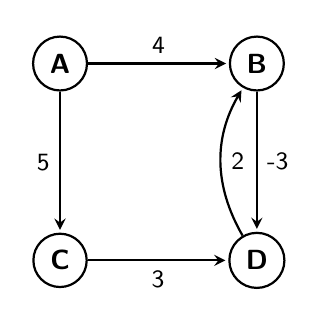
\begin{tikzpicture}[->,>=stealth,shorten >=1pt,node distance=2.5cm,
  thick,main node/.style={circle,draw,font=\sffamily\bfseries}]

  \node[main node] (1) {A};
  \node[main node] (2) [right of=1] {B};
  \node[main node] (3) [below of=1] {C};
  \node[main node] (4) [below of=2] {D};

  \path[every node/.style={font=\sffamily\small}]
    (1) edge node [above] {4} (2)
    (1) edge node [left] {5} (3)
    (2) edge node [right] {-3} (4)
    (3) edge node [below] {3} (4)
    (4) edge[bend left] node [right] {2} (2);
\end{tikzpicture}
\caption{Directed Graph with Negative Edge Weight}
\end{figure}

Vertices: A, B, C, D \\
Edges: (A, B, 4), (A, C, 5), (B, D, -3), (C, D, 3), (D, B, 2)

\subsection*{Initialization}

Source Vertex: A

\[
\begin{array}{|c|c|}
\hline
\textbf{Vertex} & \textbf{Distance from A} \\
\hline
A & 0 \\
B & \infty \\
C & \infty \\
D & \infty \\
\hline
\end{array}
\]

\subsection*{Relaxation Steps}

Bellman-Ford runs for $V-1 = 3$ iterations.

\subsubsection*{Iteration 1}

\[
\begin{array}{|c|c|l|}
\hline
\textbf{Edge} & \textbf{Relaxation} & \textbf{Updated Distances} \\
\hline
(A, B, 4) & 0 + 4 < \infty & B = 4 \\
(A, C, 5) & 0 + 5 < \infty & C = 5 \\
(B, D, -3) & 4 - 3 < \infty & D = 1 \\
(C, D, 3) & 5 + 3 > 1 & $No change$ \\
(D, B, 2) & 1 + 2 < 4 & B = 3 \\
\hline
\end{array}
\]

\textbf{Distances after Iteration 1:}
\[
A = 0,\quad B = 3,\quad C = 5,\quad D = 1
\]

\subsubsection*{Iteration 2}

\[
\begin{array}{|c|c|l|}
\hline
\textbf{Edge} & \textbf{Relaxation} & \textbf{Updated Distances} \\
\hline
(A, B, 4) & 0 + 4 > 3 & No change \\
(A, C, 5) & 0 + 5 = 5 & No change \\
(B, D, -3) & 3 - 3 = 0 < 1 & D = 0 \\
(C, D, 3) & 5 + 3 > 0 & No change \\
(D, B, 2) & 0 + 2 = 2 < 3 & B = 2 \\
\hline
\end{array}
\]

\textbf{Distances after Iteration 2:}
\[
A = 0,\quad B = 2,\quad C = 5,\quad D = 0
\]

\subsubsection*{Iteration 3}

\[
\begin{array}{|c|c|l|}
\hline
\textbf{Edge} & \textbf{Relaxation} & \textbf{Updated Distances} \\
\hline
(A, B, 4) & No change & - \\
(A, C, 5) & No change & - \\
(B, D, -3) & 2 - 3 = -1 < 0 & D = -1 \\
(C, D, 3) & No change & - \\
(D, B, 2) & -1 + 2 = 1 < 2 & B = 1 \\
\hline
\end{array}
\]

\textbf{Distances after Iteration 3:}
\[
A = 0,\quad B = 1,\quad C = 5,\quad D = -1
\]

\subsection*{Negative Cycle Check}

Run one more iteration to check if further relaxation is possible.

- Edge (B, D, -3): $1 - 3 = -2 < -1$ → \textbf{Relaxation possible!}

\[
\textcolor{red}{\textbf{Negative weight cycle detected}}
\]

---

\subsection*{Output Summary}

\begin{tcolorbox}[colback=gray!10, colframe=black, title=Result]
The graph contains a \textbf{negative weight cycle} reachable from the source. The Bellman-Ford algorithm terminates and reports failure.
\end{tcolorbox}

%%%%%%%%%%%%%%%%%%%%%%%% End Dry Run %%%%%%%%%%%%%%%%%%%%%%%%%

%%%%%%%%%%%%%%%%%%%%%%%% Explanation %%%%%%%%%%%%%%%%%%%%%%%%%%
\subsection{Understanding the Dry Run Output}

The output of the dry run simulates how the Bellman-Ford algorithm works internally. Here's what each part of the dry run means:

\subsection*{1. Step-by-Step Edge Relaxations}

Each iteration updates the shortest known distances from the source vertex (in our case, A) to all other vertices using edge relaxation.

\begin{itemize}[leftmargin=1.5em]
    \item If $dist[u] + w < dist[v]$, then $dist[v]$ is updated.
    \item This simulates checking if going through an intermediate node gives a shorter path.
\end{itemize}

For example, in Iteration 1:
\begin{itemize}
    \item Distance to B becomes 4 via A $\rightarrow$ B
    \item Distance to C becomes 5 via A $\rightarrow$ C
    \item Distance to D becomes 1 via A $\rightarrow$ B $\rightarrow$ D
\end{itemize}

\subsection*{2. Multiple Iterations Improve Paths}

Bellman-Ford runs the edge relaxation process $V-1$ times (where $V$ is the number of vertices). This ensures all shortest paths (which can be at most $V-1$ edges long) are found.

\begin{itemize}
    \item Distances improve progressively as better paths are discovered.
    \item For example: D goes from $\infty \rightarrow 1 \rightarrow 0 \rightarrow -1$
\end{itemize}

\subsection*{3. Final Iteration: Negative Cycle Detection}

After the $V-1$ iterations, Bellman-Ford runs one extra iteration to check if any edge can still be relaxed. 

\begin{itemize}
    \item If yes, then the graph contains a \textbf{negative weight cycle}.
    \item Such cycles allow endlessly reducing path costs, making shortest path meaningless.
\end{itemize}

In our example:
\[
\text{Edge (B, D, -3): } 1 - 3 = -2 < -1
\]
\[
\Rightarrow \textcolor{red}{\textbf{Negative weight cycle detected}}
\]

\subsection*{4. Final Interpretation}

\begin{table}[H]
\centering
\renewcommand{\arraystretch}{1.3}
\begin{tabular}{|p{5cm}|p{8cm}|}
\hline
\textbf{What it shows} & \textbf{Meaning in Algorithm} \\
\hline
Distance updates in each iteration & Edge relaxations updating shortest known paths \\
\hline
Improving distances over rounds & Intermediate vertices offering shorter routes \\
\hline
Negative cycle detection step & Unique ability of Bellman-Ford to identify cycles \\
\hline
Final result box output & Indicates if shortest paths are valid or undefined \\
\hline
\end{tabular}
\end{table}

\newpage
\subsection*{5. Why It Matters}

Understanding the dry run helps solve problems that ask:
\begin{itemize}
    \item How many iterations are required?
    \item Will Bellman-Ford detect a negative cycle?
    \item Which algorithm (Bellman-Ford or Dijkstra) is more suitable for a graph?
\end{itemize}

%%%%%%%%%%%%%%%%%%%%%%%%%%%%%% End %%%%%%%%%%%%%%%%%%%%%%%%%%%%

%%%%%%%%%%%%%%%%%%%%%%%%%% Positive Edge Weight %%%%%%%%%%%%%%
\subsection{Example Graph: With Positive Edge Weight}
\begin{figure}[H]
\centering
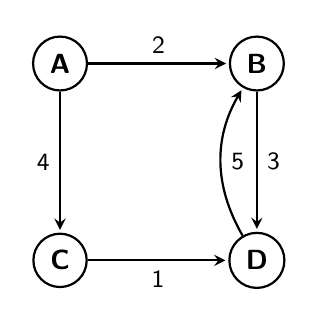
\begin{tikzpicture}[->,>=stealth,shorten >=1pt,node distance=2.5cm,
  thick,main node/.style={circle,draw,font=\sffamily\bfseries}]

  \node[main node] (A) {A};
  \node[main node] (B) [right of=A] {B};
  \node[main node] (C) [below of=A] {C};
  \node[main node] (D) [right of=C] {D};

  \path[every node/.style={font=\sffamily\small}]
    (A) edge node [above] {2} (B)
    (A) edge node [left] {4} (C)
    (B) edge node [right] {3} (D)
    (C) edge node [below] {1} (D)
    (D) edge[bend left] node [right] {5} (B); % forms a positive cycle
\end{tikzpicture}
\caption{Graph with Positive Edge Weight Cycle}
\end{figure}

\textbf{Vertices:} A, B, C, D

\textbf{Edges:} (A, B, 2), (A, C, 4), (B, D, 3), (C, D, 1), (D, B, 5)

\subsection*{Initialization}

Source Vertex: A

\[
\begin{array}{|c|c|}
\hline
\textbf{Vertex} & \textbf{Distance from A} \\
\hline
A & 0 \\
B & \infty \\
C & \infty \\
D & \infty \\
\hline
\end{array}
\]

\subsection*{Relaxation Steps (3 Iterations)}

\subsubsection*{Iteration 1}
\[
\begin{array}{|c|c|l|}
\hline
\textbf{Edge} & \textbf{Relaxation Condition} & \textbf{Updated Distances} \\
\hline
(A, B, 2) & 0 + 2 < \infty & B = 2 \\
(A, C, 4) & 0 + 4 < \infty & C = 4 \\
(B, D, 3) & 2 + 3 < \infty & D = 5 \\
(C, D, 1) & 4 + 1 = 5 \geq 5 & No change \\
(D, B, 5) & 5 + 5 = 10 > 2 & No change \\
\hline
\end{array}
\]

\textbf{After Iteration 1:}
\[
A = 0, \quad B = 2, \quad C = 4, \quad D = 5
\]

\subsubsection*{Iteration 2}
No edge relaxes further.

\textbf{All conditions fail: distances unchanged.}

\subsubsection*{Iteration 3}
Still no changes.

\[
\Rightarrow \text{All distances are stable.}
\]

\subsection*{Negative Cycle Check}

Perform one more iteration:

\begin{itemize}
  \item No edge $(u, v)$ satisfies $dist[u] + w < dist[v]$
  \item So, \textbf{no negative weight cycle exists}
\end{itemize}

% \begin{tcolorbox}[colback=green!5!white, colframe=green!80!black, title=Final Result]
\begin{tcolorbox}[colback=white, colframe=black, title=Final Result]
The graph does not contain a negative weight cycle. \\
Shortest distances from A are:
\[
\boxed{
A = 0, \quad B = 2, \quad C = 4, \quad D = 5
}
\]
\end{tcolorbox}
%%%%%%%%%%%%%%%%%%%%%%% End %%%%%%%%%%%%%%%%%%%%%%%%%%%%%%%%%%

%%%%%%%%%%%%%%%%%%% Understandint the output %%%%%%%%%%%%%%%%%%%%%%%%%%
\subsection{Understanding the Output of the Dry Run}

The dry run demonstrates how the Bellman-Ford algorithm processes graphs with only positive edge weights. Below is the interpretation of the output:

\subsection*{1. Edge Relaxation Steps}

In the first iteration, all reachable vertices from the source (A) have their distances updated because the initial distances are $\infty$. Each edge is examined and relaxed if a shorter path is found:

\begin{itemize}
    \item $(A, B, 2)$ sets $dist[B] = 2$
    \item $(A, C, 4)$ sets $dist[C] = 4$
    \item $(B, D, 3)$ sets $dist[D] = 5$
\end{itemize}

No further updates are made in subsequent iterations, which means that the shortest paths have already been found.

\subsection*{2. Stable Distances After Iteration 1}

After the first iteration, the shortest distances from the source vertex A to all other vertices are finalized:

\[
\boxed{
A = 0, \quad B = 2, \quad C = 4, \quad D = 5
}
\]

\begin{itemize}
    \item No edge caused a relaxation in iteration 2 or 3.
    \item This indicates that the shortest paths have been found before completing all $V-1$ iterations.
\end{itemize}

\subsection*{3. Cycle Handling with Positive Weights}

The graph contains a cycle: $B \rightarrow D \rightarrow B$, with total weight $3 + 5 = 8$.

\begin{itemize}
    \item Since the total weight is positive, it does not cause any endless relaxation.
    \item Bellman-Ford correctly ignores such cycles when computing shortest paths.
\end{itemize}

\subsection*{4. Final Negative Cycle Check}

After the $V-1$ iterations, Bellman-Ford checks all edges once more to see if any further relaxation is possible.

\begin{itemize}
    \item No edge satisfies $dist[u] + w < dist[v]$
    \item Therefore, \textbf{no negative weight cycle exists}
\end{itemize}

\begin{tcolorbox}[colback=white, colframe=black, title=Conclusion]
The algorithm successfully terminates. All shortest distances from source vertex A have been computed correctly, and no negative weight cycle is present in the graph.
\end{tcolorbox}

%%%%%%%%%%%%%%%%%%%%%%%%%%%%%%% End %%%%%%%%%%%%%%%%%%%%%%%%%%%%%%%%%%%
\newpage    
%%%%%%%%%%%%%%%%%%%%%%%%%% Python Code %%%%%%%%%%%%%%%%%%%%%%%%%%%%%%%%
\subsection{Python Code}
\begin{lstlisting}[style=python, caption={Bellman-Ford Algorithm in Python}]
def bellman_ford(V, edges, source):
    # Initialize distances
    dist = [float('inf')] * V
    dist[source] = 0

    # Relax all edges (V - 1) times
    for _ in range(V - 1):
        for u, v, w in edges:
            if dist[u] != float('inf') and dist[u] + w < dist[v]:
                dist[v] = dist[u] + w

    # Check for negative weight cycles
    for u, v, w in edges:
        if dist[u] != float('inf') and dist[u] + w < dist[v]:
            print("Negative weight cycle detected.")
            return None

    return dist

# Example usage
V = 4
edges = [
    (0, 1, 2),   # A -> B
    (0, 2, 4),   # A -> C
    (1, 3, 3),   # B -> D
    (2, 3, 1),   # C -> D
    (3, 1, 5)    # D -> B (positive cycle)
]
source = 0  # Vertex A
distances = bellman_ford(V, edges, source)

if distances:
    print("Shortest distances from source A:")
    for i, d in enumerate(distances):
        print(f"Vertex {chr(ord('A') + i)}: {d}")
\end{lstlisting}

\newpage
\subsection{Explanation of Bellman-Ford Algorithm in Python}

\begin{enumerate}[leftmargin=2em,label=\textbf{Line \arabic*:}]
  \item Define the function \texttt{bellman\_ford} with parameters: number of vertices \( V \), list of edges, and the source vertex.
  \item Initialize a list \texttt{dist} with \(\infty\) for all vertices, representing unreachable distances initially.
  \item Set the distance of the source vertex to 0, since the shortest path to itself is 0.
  \item Begin the relaxation phase: loop \( V-1 \) times (as per the Bellman-Ford algorithm).
  \item For each edge \((u, v, w)\), check if the distance to \( v \) through \( u \) is shorter than the current distance.
  \item If so, update \texttt{dist[v]} with the shorter distance \texttt{dist[u] + w}.
  \item After all relaxations, check again for each edge whether any further relaxation is possible.
  \item If it is, this implies a negative weight cycle exists, so print a warning and return \texttt{None}.
  \item If no negative cycles are found, return the \texttt{dist} list containing the shortest distances.
\end{enumerate}

\newpage
\subsection{Borderline Case Where Bellman-Ford Fails}

\textbf{Case: Negative Weight Cycle Reachable from the Source}

The Bellman-Ford algorithm fails when a negative weight cycle is reachable from the source vertex. This is because the algorithm relies on the fact that shortest paths can be calculated in at most \( V - 1 \) edge relaxations. However, if a cycle with total negative weight exists, the distance to some nodes can always be reduced by going around the cycle repeatedly.

\subsection*{Example}

\begin{center}
\begin{tabular}{|c|c|c|c|}
\hline
\textbf{Edge} & \textbf{From} & \textbf{To} & \textbf{Weight} \\
\hline
1 & A & B & 1 \\
2 & B & C & -1 \\
3 & C & A & -1 \\
\hline
\end{tabular}

\end{center}

This forms a cycle: A → B → C → A with total weight \( 1 + (-1) + (-1) = -1 \), which is negative.

If the source is A, Bellman-Ford will:
\begin{itemize}
    \item Relax edges for \( V-1 = 2 \) times.
    \item On the 3rd pass (for cycle detection), it will detect that further relaxation is possible: 
    \[
    \text{dist}[A] > \text{dist}[C] + w(C \rightarrow A)
    \]
    \item It prints \texttt{"Negative weight cycle detected"} and returns \texttt{None}.
\end{itemize}

\subsection*{Why This Happens}

Because in the presence of a reachable negative weight cycle:
\begin{itemize}
    \item The shortest path is not well-defined.
    \item It can be made infinitely small by repeating the cycle.
\end{itemize}

\subsection*{Important Notes}
\begin{itemize}
    \item If the cycle is not \textit{reachable} from the source, Bellman-Ford works fine.
    \item Bellman-Ford is one of the few shortest path algorithms that can even \textbf{detect} such cycles.
\end{itemize}

%%%%%%%%%%%%%%%%%%%%%%%%%%%%%%%%%%%%%%%%%%%%%%%%%%%%%%%%%%%%%%%%%%%%%%%%%%%%%%%%%%%%%%%%%%%%%%%
%%%%%%%%%%%%%%%%%%%%%%%%%%%%%% Floyd-Warshall Algorithm %%%%%%%%%%%%%%%%%%%%%%%%%%%%%%%%%%%%%%%
%%%%%%%%%%%%%%%%%%%%%%%%%%%%%%%%%%%%%%%%%%%%%%%%%%%%%%%%%%%%%%%%%%%%%%%%%%%%%%%%%%%%%%%%%%%%%%%
\newpage
\section{Floyd-Warshall Algorithm}

\subsection{Purpose}
The \textbf{Floyd-Warshall Algorithm} is used to compute the shortest paths between \textbf{all pairs of vertices} in a weighted directed graph. It works for graphs with positive and negative edge weights (but no negative weight cycles).

Common applications:
\begin{itemize}[leftmargin=1.5em]
    \item Network routing between all routers
    \item Finding transitive closures
    \item Calculating reachability in graphs
\end{itemize}

\subsection{Time Complexity}
\[
O(V^3)
\]
where \( V \) is the number of vertices. It uses three nested loops over the vertices.

\subsection{Space Complexity}
\[
O(V^2)
\]
because it stores all-pairs shortest distances in a 2D matrix.

\subsection{Key Features}
\begin{itemize}[leftmargin=1.5em]
    \item Solves the \textbf{All-Pairs Shortest Path} problem
    \item Works with \textbf{negative weights} (but not negative cycles)
    \item Uses \textbf{Dynamic Programming} to build solutions incrementally
    \item Simpler implementation than running Dijkstra \( V \) times
\end{itemize}

\newpage
\subsection{Step-by-Step Explanation}
Let \( dist[i][j] \) be the shortest distance from vertex \( i \) to vertex \( j \).

The algorithm works as follows:
\begin{enumerate}[leftmargin=1.5em]
    \item Initialize the distance matrix:
    \[
    dist[i][j] = \begin{cases}
        0 & \text{if } i = j \\
        \text{weight}(i, j) & \text{if } (i, j) \in E \\
        \infty & \text{otherwise}
    \end{cases}
    \]
    \item For each vertex \( k \), update:
    \[
    \text{If } dist[i][k] + dist[k][j] < dist[i][j] \text{ then set } dist[i][j] = dist[i][k] + dist[k][j]
    \]
    \item Repeat this for all \( k \in [1, V] \)
\end{enumerate}

\begin{algorithm}[H]
\caption{Floyd-Warshall Algorithm}
\begin{algorithmic}[1]
\State \textbf{Input:} Weighted graph $G = (V, E)$ as adjacency matrix
\State \textbf{Output:} Matrix $dist$ of shortest distances between all pairs

\Function{FloydWarshall}{$G$}
    \State $dist \gets$ adjacency matrix of $G$
    
    \For{each vertex $k$ in $V$}
        \For{each vertex $i$ in $V$}
            \For{each vertex $j$ in $V$}
                \If{$dist[i][k] + dist[k][j] < dist[i][j]$}
                    \State $dist[i][j] \gets dist[i][k] + dist[k][j]$
                \EndIf
            \EndFor
        \EndFor
    \EndFor
    
    \State \Return $dist$
\EndFunction
\end{algorithmic}
\end{algorithm}

\subsection{Comparison with Dijkstra's Algorithm}
\begin{table}[H]
\centering
\renewcommand{\arraystretch}{1.3}
\begin{tabular}{|p{5.2cm}|p{5.5cm}|p{5.5cm}|}
\hline
\textbf{Feature} & \textbf{Floyd-Warshall} & \textbf{Dijkstra} \\
\hline
Problem Type & All-pairs shortest path & Single-source shortest path \\
\hline
Time Complexity & $O(V^3)$ & $O((V+E)\log V)$ (with min-heap) \\
\hline
Handles Negative Weights & Yes & No (fails for negative weights) \\
\hline
Negative Cycle Detection & No (but can be checked manually) & No \\
\hline
Graph Type & Dense & Sparse \\
\hline
Approach & Dynamic Programming & Greedy + Min-Heap \\
\hline
Ease of Implementation & Very simple & More complex with heap \\
\hline
\end{tabular}
\end{table}

\section{Dry Run: Floyd-Warshall Algorithm}

\subsection{Example Graph: With Negative Edge Weight}
\begin{figure}[H]
\centering
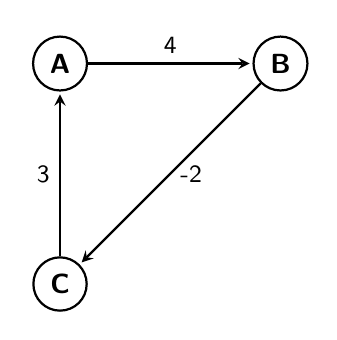
\begin{tikzpicture}[->,>=stealth,shorten >=1pt,node distance=2.8cm, thick,
  main node/.style={circle,draw,font=\sffamily\bfseries}]
  
  \node[main node] (A) {A};
  \node[main node] (B) [right of=A] {B};
  \node[main node] (C) [below of=A] {C};

  \path[every node/.style={font=\sffamily\small}]
    (A) edge node[above] {4} (B)
    (B) edge node[right] {-2} (C)
    (C) edge node[left] {3} (A);
\end{tikzpicture}
\caption{Graph with Negative Edge Weight (No negative cycle)}
\end{figure}

Vertices: A = 0, B = 1, C = 2

Edges:
\[
(0, 1, 4),\quad (1, 2, -2),\quad (2, 0, 3)
\]

\newpage
\textbf{Initial Distance Matrix:}
\[
\begin{bmatrix}
0 & 4 & \infty \\
\infty & 0 & -2 \\
3 & \infty & 0 \\
\end{bmatrix}
\]

\textbf{After k=0:}
\[
\text{No changes (only self-loops)}
\]

\textbf{After k=1:}
\[
dist[0][2] = dist[0][1] + dist[1][2] = 4 + (-2) = 2
\]

\textbf{After k=2:}
\[
dist[1][0] = dist[1][2] + dist[2][0] = -2 + 3 = 1
\]
\[
dist[1][1] = dist[1][0] + dist[0][1] = 1 + 4 = 5
\]

\subsection{Understanding the Dry Run Output}

\begin{itemize}[leftmargin=1.5em]
    \item Floyd-Warshall computes the shortest path between all node pairs.
    \item It progressively improves the solution by considering each vertex as an intermediate step.
    \item Negative edge weights are handled properly, as long as there are no negative cycles.
    \item If any $dist[i][i] < 0$ at the end, a \textbf{negative cycle} is detected.
\end{itemize}

\begin{tcolorbox}[colback=white, colframe=black, title=Final Result (Negative Edge)]
Shortest path matrix is successfully computed with negative weights (no cycle).
\end{tcolorbox}

\newpage
\subsection{Example Graph: With Positive Edge Weight}
\begin{figure}[H]
\centering
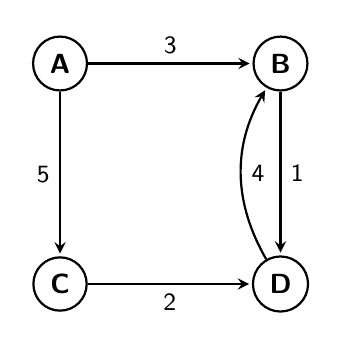
\begin{tikzpicture}[->,>=stealth,shorten >=1pt,node distance=2.8cm, thick,
  main node/.style={circle,draw,font=\sffamily\bfseries}]
  
  \node[main node] (A) {A};
  \node[main node] (B) [right of=A] {B};
  \node[main node] (C) [below of=A] {C};
  \node[main node] (D) [right of=C] {D};

  \path[every node/.style={font=\sffamily\small}]
    (A) edge node[above] {3} (B)
    (A) edge node[left] {5} (C)
    (B) edge node[right] {1} (D)
    (C) edge node[below] {2} (D)
    (D) edge[bend left] node[right] {4} (B);
\end{tikzpicture}
\caption{Graph with Positive Edge Weights}
\end{figure}

\textbf{Vertices:} A = 0, B = 1, C = 2, D = 3

\textbf{Initial Distance Matrix:}
\[
\begin{bmatrix}
0 & 3 & 5 & \infty \\
\infty & 0 & \infty & 1 \\
\infty & \infty & 0 & 2 \\
\infty & 4 & \infty & 0 \\
\end{bmatrix}
\]

\subsection{Understanding the Output of the Dry Run}

\begin{itemize}
    \item After multiple updates, all indirect shortest paths are computed.
    \item The algorithm detects no negative cycles.
    \item Final matrix contains the shortest distances between all vertex pairs.
\end{itemize}

\begin{tcolorbox}[colback=white, colframe=black, title=Final Result (Positive Edges)]
All-pairs shortest paths successfully computed with only positive weights.
\end{tcolorbox}

\newpage
\subsection{Python Code}
\begin{lstlisting}[style=python, caption={Floyd-Warshall Algorithm in Python}]
def floyd_warshall(V, edges):
    dist = [[float('inf')] * V for _ in range(V)]

    for i in range(V):
        dist[i][i] = 0

    for u, v, w in edges:
        dist[u][v] = w

    for k in range(V):
        for i in range(V):
            for j in range(V):
                if dist[i][k] + dist[k][j] < dist[i][j]:
                    dist[i][j] = dist[i][k] + dist[k][j]

    # Optional: detect negative cycles
    for i in range(V):
        if dist[i][i] < 0:
            print("Negative weight cycle detected.")
            return None

    return dist

# Example usage:
edges = [
    (0, 1, 3),  # A -> B
    (0, 2, 5),  # A -> C
    (1, 3, 1),  # B -> D
    (2, 3, 2),  # C -> D
    (3, 1, 4)   # D -> B
]
dist = floyd_warshall(4, edges)
for i, row in enumerate(dist):
    print(f"From {chr(65+i)}:", row)
\end{lstlisting}

\newpage
\subsection{Explanation of Floyd-Warshall Algorithm (Python)}

\begin{enumerate}[leftmargin=2em]
    \item \texttt{def floyd\_warshall(V, edges):} \\
    Defines a function that takes the number of vertices \(V\) and a list of edges. Each edge is a tuple \((u, v, w)\) representing an edge from \(u\) to \(v\) with weight \(w\).

    \item \texttt{dist = [[float('inf')] * V for \_ in range(V)]} \\
    Initializes a \(V \times V\) distance matrix with \(\infty\), meaning all distances are initially unknown.

    \item \texttt{for i in range(V):} \\
    Loop over all vertices to set distance from a vertex to itself as 0.

    \item \texttt{dist[i][i] = 0} \\
    The shortest distance from any vertex to itself is 0.

    \item \texttt{for u, v, w in edges:} \\
    Iterates over each edge in the input edge list.

    \item \texttt{dist[u][v] = w} \\
    Updates the matrix with the given edge weights.

    \item \texttt{for k in range(V):} \\
    Outer loop over all vertices \(k\). This represents intermediate nodes in the path.

    \item \texttt{for i in range(V):} \\
    Inner loop for source vertices.

    \item \texttt{for j in range(V):} \\
    Inner loop for destination vertices.

    \item \texttt{if dist[i][k] + dist[k][j] < dist[i][j]:} \\
    If the path from \(i\) to \(j\) via \(k\) is shorter than the current known path, update it.

    \item \texttt{dist[i][j] = dist[i][k] + dist[k][j]} \\
    Update the shortest distance from \(i\) to \(j\) using \(k\) as an intermediate.

    \item \texttt{for i in range(V):} \\
    After all updates, check for negative weight cycles.

    \item \texttt{if dist[i][i] < 0:} \\
    If the diagonal of the matrix is negative, it indicates a negative weight cycle involving vertex \(i\).

    \item \texttt{print("Negative weight cycle detected.")} \\
    Warn the user about the presence of a negative cycle.

    \item \texttt{return None} \\
    Abort and return \texttt{None} to indicate failure.

    \item \texttt{return dist} \\
    If no negative cycle is found, return the final distance matrix.
\end{enumerate}

\subsection{Borderline Case: When Floyd-Warshall Fails}

\textbf{Case: Graph with a Negative Weight Cycle}

The Floyd-Warshall algorithm fails to compute valid shortest paths when a \textbf{negative weight cycle} exists in the graph.

\subsection*{Why it Fails}
\begin{itemize}[leftmargin=2em]
    \item In a negative cycle, you can loop through the cycle indefinitely to reduce the total path cost.
    \item As a result, the concept of a "shortest path" is not well-defined.
    \item Floyd-Warshall relies on dynamic programming assuming that once the shortest path between any two nodes is found, it cannot get shorter — this assumption breaks in the presence of negative cycles.
\end{itemize}

\subsection*{How to Detect It}
\begin{itemize}[leftmargin=2em]
    \item After running the algorithm, check the diagonal entries of the distance matrix:
    \[
        \text{If } dist[i][i] < 0 \text{ for any } i, \text{ a negative cycle exists.}
    \]
\end{itemize}

\subsection*{Example}
A graph with the following edges:
\begin{itemize}
    \item A → B (weight = 1)
    \item B → C (weight = -2)
    \item C → A (weight = -2)
\end{itemize}

\vspace{1cm}
Forms a cycle A → B → C → A with 
\begin{center}
    total weight = \(1 + (-2) + (-2) = -3\). 
\end{center}
\hspace{0.8cm}This is a negative cycle.


\textbf{Floyd-Warshall will detect this because:}
\[
    dist[A][A] = -3 < 0
\]

\textbf{Hence, result is invalid and must be discarded.}

% \begin{tcolorbox}[colback=white, colframe=black, title= , sharp corners, boxrule=0.5pt]
\subsection{Logic to Detect Negative Weight Cycles}

The Floyd-Warshall algorithm detects negative weight cycles by analyzing the final values in the distance matrix.

\textbf{Key Observations:}
\begin{itemize}[leftmargin=2em]
    \item Initially, the diagonal entries of the distance matrix are all set to 0: \\
    \[
    \texttt{dist[i][i] = 0} \quad \text{for all } i
    \]
    
    \item During the algorithm's execution, the matrix is updated using:
    \[
    \texttt{dist[i][j] = min(dist[i][j], dist[i][k] + dist[k][j])}
    \]

    \item If a node can reach itself with a total cost less than 0, then a negative weight cycle exists.
\end{itemize}

\textbf{Detection Condition:}
\[
\exists\, i \in V \text{ such that } \texttt{dist[i][i] < 0}
\]

\textbf{Interpretation:}
\begin{itemize}[leftmargin=2em]
    \item This means there exists a cycle starting and ending at node \(i\) with negative total weight.
    \item The algorithm will detect this and report the cycle if such a condition is found.
\end{itemize}

\textbf{Conclusion:} If any diagonal entry of the final distance matrix is negative, the graph contains a negative weight cycle, and shortest paths are undefined.



\newpage
% \vspace{5cm}
%%%%%%%%%%%%%%%%%%%%%%%%%%%%%% Key Points %%%%%%%%%%%%%%%%%%%%%%%%%%%%%%%%%%%%%
\section{10 Key Points:}
\subsection{Bellman-Ford Algorithm}
\begin{enumerate}[leftmargin=1.5em, label=\textbf{\arabic*.}]
    \item Solves \textbf{Single-Source Shortest Path} (SSSP) problem.
    \item Works with \textbf{negative edge weights}.
    \item Detects \textbf{negative weight cycles}.
    \item Time Complexity: \( O(V \cdot E) \).
    \item Uses \textbf{edge relaxation} process up to \( V - 1 \) times.
    \item Final pass checks for further relaxation to detect cycles.
    \item Works for both \textbf{directed} and \textbf{undirected} graphs.
    \item Distance array initialized with \( \infty \); source = 0.
    \item Slower than Dijkstra but more versatile.
    \item Common in scenarios with possible \textbf{debt or penalties}.
\end{enumerate}

\vspace{1em}

\subsection{Floyd-Warshall Algorithm}
\begin{enumerate}[leftmargin=1.5em, label=\textbf{\arabic*.}]
    \item Solves \textbf{All-Pairs Shortest Path} (APSP) problem.
    \item Based on \textbf{dynamic programming}.
    \item Handles \textbf{negative edge weights}, not negative cycles.
    \item Time Complexity: \( O(V^3) \).
    \item Space Complexity: \( O(V^2) \) using a 2D matrix.
    \item Initializes distance matrix with direct edge weights.
    \item Triple nested loop updates all distances.
    \item Simple to implement; good for \textbf{dense graphs}.
    \item Can be used to detect negative cycles via diagonal \( dist[i][i] < 0 \).
    \item Used in \textbf{network routing}, \textbf{transitive closure}, etc.
\end{enumerate}

% \begin{table}[H]
% \centering
% \renewcommand{\arraystretch}{1.4}
% \begin{tabular}{|p{7.3cm}|p{7.3cm}|}
% \hline
% \textbf{Bellman-Ford Algorithm} & \textbf{Floyd-Warshall Algorithm} \\
% \hline
% 1. Solves \textbf{Single-Source\newline Shortest Path} (SSSP) problem. & 1. Solves \textbf{All-Pairs Shortest Path} (APSP) problem. \\
% 2. Works with \textbf{negative edge weights}. & 2. Based on \textbf{dynamic\newline programming}. \\
% 3. Detects \textbf{negative weight\newline cycles}. & 3. Handles \textbf{negative edge weights}, not negative cycles. \\
% 4. Time Complexity: \(O(V \cdot E)\). & 4. Time Complexity: \(O(V^3)\). \\
% 5. Uses \textbf{edge relaxation} up to \(V - 1\) times. & 5. Space Complexity: \(O(V^2)\)\newline using a 2D matrix. \\
% 6. Final pass detects cycles by\newline further relaxation. & 6. Initializes matrix with direct edge weights. \\
% 7. Works for \textbf{directed} and\newline \textbf{undirected} graphs. & 7. Triple nested loop updates all distances. \\
% 8. Distance array starts with \(\infty\); source = 0. & 8. Good for \textbf{dense graphs},\newline simple to implement. \\
% 9. Slower than Dijkstra but more flexible. & 9. Can detect negative cycles via \(dist[i][i] < 0\). \\
% 10. Used in cases with \textbf{debt, penalties}, etc. & 10. Used in \textbf{routing}, \textbf{transitive closure}, etc. \\
% \hline
% \end{tabular}
% \caption{Comparison of Key Points: Bellman-Ford vs Floyd-Warshall Algorithm}
% \end{table}


\newpage
\section{Final Summary: Bellman-Ford vs Floyd-Warshall}

\begin{tcolorbox}[colback=white, colframe=black, title=Bellman-Ford Algorithm Summary]
\begin{itemize}[leftmargin=1.5em]
    \item Solves \textbf{Single-Source Shortest Path (SSSP)} problem.
    \item Works with \textbf{negative weights} and \textbf{detects negative cycles}.
    \item Time Complexity: \( O(V \cdot E) \)
    \item Uses \textbf{edge relaxation} repeated \( V - 1 \) times.
    \item Ideal for graphs with negative weights and when only one source is given.
\end{itemize}
\end{tcolorbox}

\vspace{0.5em}

\begin{tcolorbox}[colback=white, colframe=black, title=Floyd-Warshall Algorithm Summary]
\begin{itemize}[leftmargin=1.5em]
    \item Solves \textbf{All-Pairs Shortest Path (APSP)} problem.
    \item Handles \textbf{negative edge weights} (not cycles).
    \item Time Complexity: \( O(V^3) \)
    \item Based on \textbf{dynamic programming} and a distance matrix.
    \item Useful in dense graphs and applications like routing, transitive closure.
\end{itemize}
\end{tcolorbox}

\vspace{1em}

\begin{table}[H]
\centering
\renewcommand{\arraystretch}{1.3}
\begin{tabular}{|p{5cm}|p{5.5cm}|p{5.5cm}|}
\hline
\textbf{Aspect} & \textbf{Bellman-Ford} & \textbf{Floyd-Warshall} \\
\hline
Problem Solved & Single-source shortest path & All-pairs shortest path \\
\hline
Handles Negative Weights & Yes & Yes \\
\hline
Negative Cycle Detection & Yes & Via diagonal check: \( dist[i][i] < 0 \) \\
\hline
Time Complexity & \( O(V \cdot E) \) & \( O(V^3) \) \\
\hline
Approach & Edge relaxation & Dynamic programming \\
\hline
Graph Type & Directed / undirected & Directed (preferably dense) \\
\hline
Use Case & When source node is known & When all node pairs matter \\
\hline
\end{tabular}
\caption{Comparison Summary: Bellman-Ford vs Floyd-Warshall}
\end{table}

\newpage

% \section{Comparison}

\renewcommand{\arraystretch}{1.4}
% \begin{table}[H]
\begin{table}[ht]
\centering
\begin{tabularx}{\textwidth}{|>{\raggedright\arraybackslash}p{4.2cm}|
                            >{\raggedright\arraybackslash}X|
                            >{\raggedright\arraybackslash}X|
                            >{\raggedright\arraybackslash}X|}
\hline
\textbf{Feature} & \textbf{Bellman-Ford} & \textbf{Dijkstra} & \textbf{Floyd-Warshall} \\
\hline
\textbf{Problem Type} & Single-source shortest path (SSSP) & Single-source shortest path (SSSP) & All-pairs shortest path (APSP) \\
\hline
\textbf{Graph Type} & Directed / Undirected & Directed / Undirected & Directed \\
\hline
\textbf{Negative Weights} & Supported & Not supported & Supported (no negative cycles) \\
\hline
\textbf{Negative Cycle Detection} & Yes & No & Can be checked via \(dist[i][i] < 0\) \\
\hline
\textbf{Time Complexity} & \(O(V \cdot E)\) & \(O((V + E)\log V)\)\newline (with heap) & \(O(V^3)\) \\
\hline
\textbf{Space Complexity} & \(O(V)\) & \(O(V)\) & \(O(V^2)\) \\
\hline
\textbf{Algorithm Type} & Edge Relaxation (DP-based) & Greedy + Min-Heap & Dynamic Programming Matrix \\
\hline
\textbf{Ease of Implementation} & Easy & Medium (with heap) & Very Easy \\
\hline
\textbf{Best for} & Graphs with negative weights / cycle detection & Sparse graphs & Dense graphs / APSP \\
\hline
\textbf{Path Reconstruction} & Parent array & Parent array & Predecessor matrix (optional) \\
\hline
\end{tabularx}
\caption{Comparison Summary: Bellman-Ford vs Dijkstra vs Floyd-Warshall}
\end{table}


\end{document}
